\documentclass[12pt, a4paper]{article}

\usepackage[utf8]{inputenc}
% Limit the page margin to only 1 inch.
\usepackage[margin=1in]{geometry}

%Imports biblatex package
\usepackage[
backend=biber,
style=alphabetic
]{biblatex}
\addbibresource{../../algs4e.bib}

% Enables the `align' environment.
\usepackage{amsmath}
% Provides useful environments, such as:
% - \begin{proof} ...\end{proof}
\usepackage{amsthm}
\usepackage[most]{tcolorbox}

\newtheorem*{proposition}{Proposition}

% Enables using \mathbb{}, for example \mathbb{N} for the set of natural numbers.
\usepackage{amssymb}

% Allows using letters in enumerate list environment. Use, for example:
%\begin{enumerate}[label=(\alph*)]
% ...
%\end{enumerate}
\usepackage[inline]{enumitem}

% Enable importing external graphic files and provides useful commannds, like \graphicspath{}
\usepackage{graphicx}
% Images are located in a directory called images in the current directory.
\graphicspath{{./images/}}

% Make links look better by default.
% See: https://tex.stackexchange.com/questions/823/remove-ugly-borders-around-clickable-cross-references-and-hyperlinks
\usepackage[hidelinks]{hyperref}
\usepackage{xcolor}
\hypersetup{
	colorlinks,
	linkcolor={red!50!black},
	citecolor={blue!50!black},
	urlcolor={blue!80!black}
}


% Code Listings. Source:
% https://stackoverflow.com/questions/3175105/inserting-code-in-this-latex-document-with-indentation
\usepackage{listings}
\usepackage{color}

\definecolor{dkgreen}{rgb}{0,0.6,0}
\definecolor{gray}{rgb}{0.5,0.5,0.5}
\definecolor{mauve}{rgb}{0.58,0,0.82}

\lstset{frame=tb,
	language=Java,
	aboveskip=3mm,
	belowskip=3mm,
	showstringspaces=false,
	columns=flexible,
	basicstyle={\small\ttfamily},
	numbers=none,
	numberstyle=\tiny\color{gray},
	keywordstyle=\color{blue},
	commentstyle=\color{dkgreen},
	stringstyle=\color{mauve},
	breaklines=true,
	breakatwhitespace=true,
	tabsize=3
}

\newcommand{\prob}{\text{P}}
%\newcommand{\complement}{\mathsf{c}}

% Define an environment called "ex" (for Exercise) so that I can do: \begin{ex}{1.5}...\end{ex}
\newenvironment{ex}[2][Exercise]
{\par\medskip\noindent \textbf{#1 #2.}}
{\medskip}

% Define a solution environment, similar to ex (exercise) environment.
\newenvironment{sol}[1][Solution]
{\par\medskip\noindent \textbf{#1.} }
{\medskip}

\begin{document}
	\noindent Sergio E. Garcia Tapia \hfill
	
	\noindent \emph{Algorithms} by Sedgewick and Wayne (4th edition) \cite{sedgewick_wayne}\hfill
	
	\noindent January 25, 2025\hfill 
	\section*{5.3: Substring Search}
	\subsection*{Notes}
	To construct the \texttt{dfa[][]} array that corresponds to a pattern, the idea is to first
	fill in the match transitions. Note that \texttt{dfa[pat.charAt(j)][j]} is always \texttt{j+1}
	because if we are in state \texttt{j} (we have seen \texttt{j} characters \texttt{pat.charAt(0..j-1)}
	in the pattern) and see \texttt{pat.charAt(j)}, then we matched. Then, the challenge is
	to understand the mismatch transitions. As explained in \cite{sedgewick_wayne}, the key is
	to track what state the DFA would be in if we had a mismatch and had to back up.
	
	Say we mismatch when reading \texttt{txt.charAt(i)} while in state \texttt{j}. This
	means that the first \texttt{j} characters matched, but not the \texttt{j+1}-th character,
	so the substring does not match at position \texttt{i-j} of the text. Since we have
	seen \texttt{pat.charAt(0..j-1)} of the pattern in the text, we can use those characters
	to decide which state to backup to. If we were to back up in the brute-force method, we
	would move back to \texttt{txt.charAt(i-j+1)}, which corresponds to \texttt{pat.charAt(1)}.
	Then, we would check \texttt{pat.charAt(1..j-1)}, the pattern characters that we know occur
	in the text, and use them to figure out how where to restart.
	
	Say we are in state \texttt{5} and encountered a mismatch with a character \texttt{c}
	that does not match \texttt{pat.charAt(5)}. If we backed up, we would process characters
	\texttt{pat.charAt(1..4)} in the DFA from the beginning, and end up at a state
	\texttt{x}, called the \emph{restart state} \texttt{x} corresponding to state \texttt{5}.
	Now on processing \texttt{c} at state \texttt{5}, we transition to where the DFA
	would go when receiving \texttt{c} while in state \texttt{x}.
	\subsubsection*{Exercises}
	\begin{ex}{2}
		Give the \texttt{dfa[][]} array for the Knuth--Morris--Pratt algorithm for the pattern
		\texttt{A A A A A A A A A}, and draw the DFA, in the style of the figures in the text.
	\end{ex}
	\begin{sol}
		See Figure~\ref{fig:ex-02}. Notice that receiving any character that is not \texttt{A}
		would reset us to state \texttt{0}.
		\begin{figure}
			\centering
			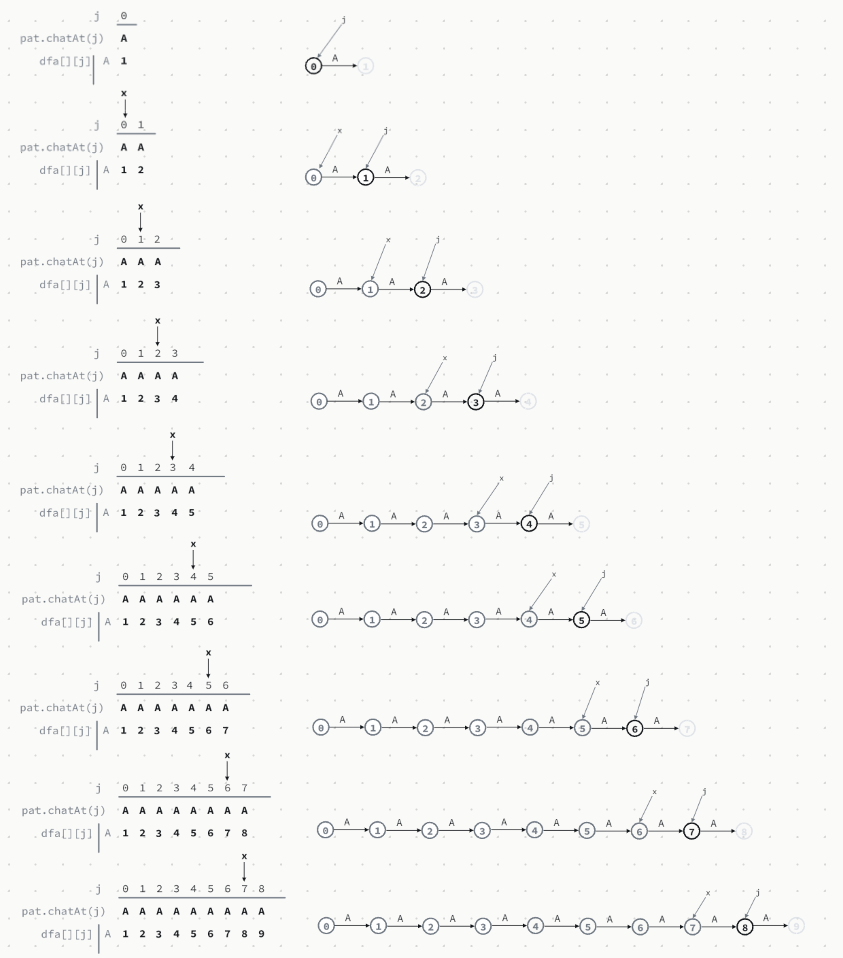
\includegraphics[width=1.0\textwidth]{exercise-02}
			\caption{Constructing the DFA For KMP substring search in Exercise 2.}
			\label{fig:ex-02}
		\end{figure}
	\end{sol}
	
	
	\pagebreak
	\printbibliography
\end{document}